\section{Theoretische Grundlagen}

\subsection{$\alpha$-Zerfall}
Als $\alpha$-Zerfall bezeichnet man den Zerfall eines Atoms, bei dem ein \atom{4}{2}{He} Ion den Kern verlässt. Die Reaktionsgleichung lautet also:
$$ \atom{A}{Z}{X} \rightarrow \atom{A-4}{Z-2}{Y}^{-2} + \atom{4}{2}{He}^{+2} $$

\atom{4}{2}{He} besitzt sowohl eine voll besetzte Neutronen- als auch eine voll besetzte Protononenschale, man bezeichnet es auch als "`doppelt magisch"', und hat somit eine sehr hohe Bindungsenergie. Klassisch betrachtet kann ein solches Ion den Atomkern dennoch nicht verlassen, da seine Energie niedriger ist als die des Coulombwalls. Quantenmechanisch ist dies natürlich durch den Tunneleffekt durchaus möglich. Die Wahrscheinlichkeit für einen $\alpha$-Zerfall ergibt sich aus dem Produkt der Einzelwahrscheinlichkeiten für die Bildung eines solchen Ions, seine Rate der "`Wallberührung"' sowie schließlich der Tunnelwahrscheinlichkeit:
$$ W = W_0 \times W_1 \times T $$
Die Tunnelwahrscheinlichkeit $T$ kann mit den Gamow-Faktor $G$ näherungsweise analytisch berechnet werden und ist unter anderem abhängig von der Wallbreite und -höhe. 

Die Energie des $\alpha$-Teilchens ergibt sich aus der Energiedifferenz zwischen Mutteratom und Tochteratom. Diese unterscheidet sich bei Zerfällen des selben Isotops höchstens durch angeregte Kernzustände. Beim Übergang vom angeregten Mutteratom zum Grundzustand des Tochteratoms erhält das Ion die höchste Energie, beim Übergang von Grundzustand zu Grundzustand ist sie etwas niedriger und für den Übergang von Grundzustand zu angeregtem Tochteratom ist sie am niedrigsten.

Da es also nur endlich viele diskrete Übergangsmöglichkeiten gibt, ist auch das Energiespektrum des $\alpha$-Zerfalls diskret.  

\subsection{$\beta$ - Zerfall}
Als $\beta$-Zerfall bezeichnet man den Übergang eines Protonen zu einem Neutronen oder eines Neutrons zu einem Proton. Der $\beta^-$-Zerfall wird beschrieben durch:
$$ \atom{A}{Z}{X} \rightarrow \atom{A}{Z+1}{Y} + e^- + \overline{\nu} $$
also
$$ n \rightarrow p + e^- + \overline{\nu_e} $$
Der $\beta^+$-Zerfall ist der Zerfall eines Protons in ein Neutron:
$$p \rightarrow n + e^+ + \nu_e$$

\subsection{Elektroneneinfang}

Als weitere Art des $\beta$-Zerfall zählt man noch den Elektroneneinfang (EC, \emph{electron capture)}. Bei diesem wird ein Elektron durch den Kern eingefangen und kombiniert mit einem Proton zu einem Neutron. Dabei wird weiterhin ein Elektronenneutrino emittiert. Am häufisten werden dabei 1s-Elektronen verwendet, da sie eine hohe Aufenthaltswahrscheinlichkeit im Kern besitzen.

$$ EC: p^+ + e^- \rightarrow n^0 + \nu_e $$

Der Elektroneneinfang gewinnt mit größeren Kernzahlen an Bedeutung, da dann die Aufenthaltswahrscheinlichkeit im Kern immer größer wird.


\subsection{$\gamma$-Strahlung}

Zerfällt ein Atom beim $\alpha$- und $\beta$-Zerfall in einen angeregten Tochterzustand, so geht dieses innerhalb einer sehr kurzen Zeit ($\sim 10^-9 bis 10^-12 s$) in den Grundzustand über. Dabei wird entweder ein Photon emittiert, genannt $\gamma$-Quant, oder es findet \paragraph{Innere Konversion} statt. Die Energie des Kerns geht an ein Hüllenelektron, welches dadurch das Atom mit der verbleibenden Energie als kinetische Energie verlässt. Diese Elektronenlücke wird durch ein Elektron aus einer höheren Schale ersetzt, welches seine überschüssige Energie durch ein Photon (bei schweren Elementen) oder den \paragraph{Auger-Effekt} (bei leichten Elementen) abgiebt.
Dies bedeutet, dass die überschüssige Energie wiederum an ein Elektron abgegeben wird, welches dadurch das Atom verlässt und damit ein zweites Loch im Atom hinterlässt.

\subsection{Zerfallsgesetz}

Radioaktive Zerfälle sind ein statistischer Prozess und können durch das Zerfallsgesetz beschrieben werden:
\begin{gather}
 \frac{dP}{dt} = \lambda \\
 \frac{dN}{dt} = - \lambda N(t) = - A(t) \label{dNdtlambdaN}\\
 N(t) = N_0 e^{-\lambda t}
\end{gather}

Daraus ergibt sich auch die Halbwertszeit:
\begin{gather}
 N(t_{1/2}) = \frac{1}{2} N_0 = N_0 e^{-\lambda t_{1/2}} \\
 \frac{1}{2} = e^{-\lambda t_{1/2}} \\
 \ln \frac{1}{2} = - \lambda t_{1/2} \\
 t_{1/2} = \frac{\ln 2}{\lambda} \label{t12ln2lambda}\\
\end{gather}

\subsection{Wechselwirkung von geladenen Teilen mit Materie}

Geladene Teilchen zeigen elektromagnetische Wechselwirkung mit den Elektronen und Kernen der Materie. Sie können entweder abgelenkt werden, wodurch Bremsstrahlung entsteht oder es kommt zu inelastischer Streuung.

\subsubsection{Bremsstrahlung}
Bremsstrahlung tritt auf, wenn die Bahn eines Teilchens geändert wird. Bei geladenen Teilchen wird dies durch die Compton-Felder der Teilchen der Materie verursacht. Für die in Form von Photonen abgegebene Energie gilt
\begin{equation}
 - \frac{dE}{dx} \rvert_{Brems.} = \frac{E}{X_0}
\end{equation}
wobei $X_0$ die materialabhängige Strahlungslänge ist und angibt, nach welcher Schichtdicke die verbleibende Energie auf $1/e \cdot E_0$ reduziert wurde.

\subsubsection{Ionisation und Anregung}
Durchqueren geladene Teilchen Materie, so können sie dort Atome und Moleküle anregen und je nach Energie auch Ionisieren. Dabei kann an ein Elektron der Materie maximal die Energie
\begin{equation}
 E_{kin}^{max} = 2 m_e v^2 \gamma^2
\end{equation}
abgegeben werden. (Wobei $v$ die Geschwindigkeit des Teilchens und $\gamma = E / m_0 c^2$ der Lorentzfaktor ist.)

Der mittlere Energieverlust $dE$ pro Wegstrecke $dx$ kann nach Bethe und Bloch berechnet werden und lautet für $\alpha$-Teilchen
\begin{equation}
 - \frac{dE}{dx} \rvert_{Ionisation} = 4 \cdot \pi \cdot \rho \cdot N_A \cdot \frac{Z}{A} \cdot \frac{z^2e^4}{m_e v^2} \cdot \ln \left[ \left( \frac{2m_ev^2}{I} \right) - \ln \left( 1- \beta^2 \right) - \beta^2 \right]
\end{equation}
mit der Ladung des Teilchens $z = 2$ und $I \simeq 13.5 eV \cdot Z$ dem mittleren Ionisationspotential.

Für die Elektronen und Positronen des $\beta$-Zerfalls müssen noch weitere Effekte berücksichtigt werden und es ergibt sich für $ E < 0.5 MeV$
\begin{equation}
 - \frac{dE}{dx} \rvert_{Ionisation} = 4 \cdot \pi \cdot \rho \cdot N_A \cdot \frac{Z}{A} \cdot \frac{z^2e^4}{m_e v^2} \cdot \ln \left( \frac{1.66 \cdot m_ev^2}{2 \cdot I} \right)
\end{equation}

sowie für $ E >> 0.5 MeV$, da diese relativistisch betrachtet werden müssen
\begin{equation}
 - \frac{dE}{dx} \rvert_{Ionisation} = 4 \cdot \pi \cdot \rho \cdot N_A \cdot \frac{Z}{A} \cdot \frac{z^2e^4}{m_e v^2} \cdot  \left[ \ln \left( \frac{E}{2 \cdot m_e \cdot c^2 \cdot I} \right) + \frac{1}{8} \right]
\end{equation}

\subsubsection{Totaler Energieverlust und Reichweite}

Summiert man die Energieverluste durch die einzelnen Prozesse so erhält man den totalen Energieverlust
\begin{equation}
 - \frac{dE}{dx} \rvert_{Total} = - \frac{dE}{dx} \rvert_{Ionisation} - \frac{dE}{dx} \rvert_{Brems.} - \frac{dE}{dx} \rvert_{Cherenkov}
\end{equation}
Dieser ergibt sich bei niedrigen Energien hauptsächlich aus der Ionisation, bei hohen Energien hingegen haupsächlich aus der Bremsstrahlung. Aus ihm kann man die Reichweite eines Teilchens berechnen, also die Strecke nach der es seine komplette Energie verloren hat
\begin{equation}
 R = \int_E^0 - \frac{dE}{dE/dx}
\end{equation}.

Diese Reichweite ist für $\alpha$-Teilchen extrem gering, wodurch die Selbstabsorbtion in der Probe sehr wichtig wird. Die Reichweite von $\beta$-Strahlung ist hingegen deutlich größer.  


\subsection{Durchflusszählrohr}
\begin{figure}[H]
 \centering 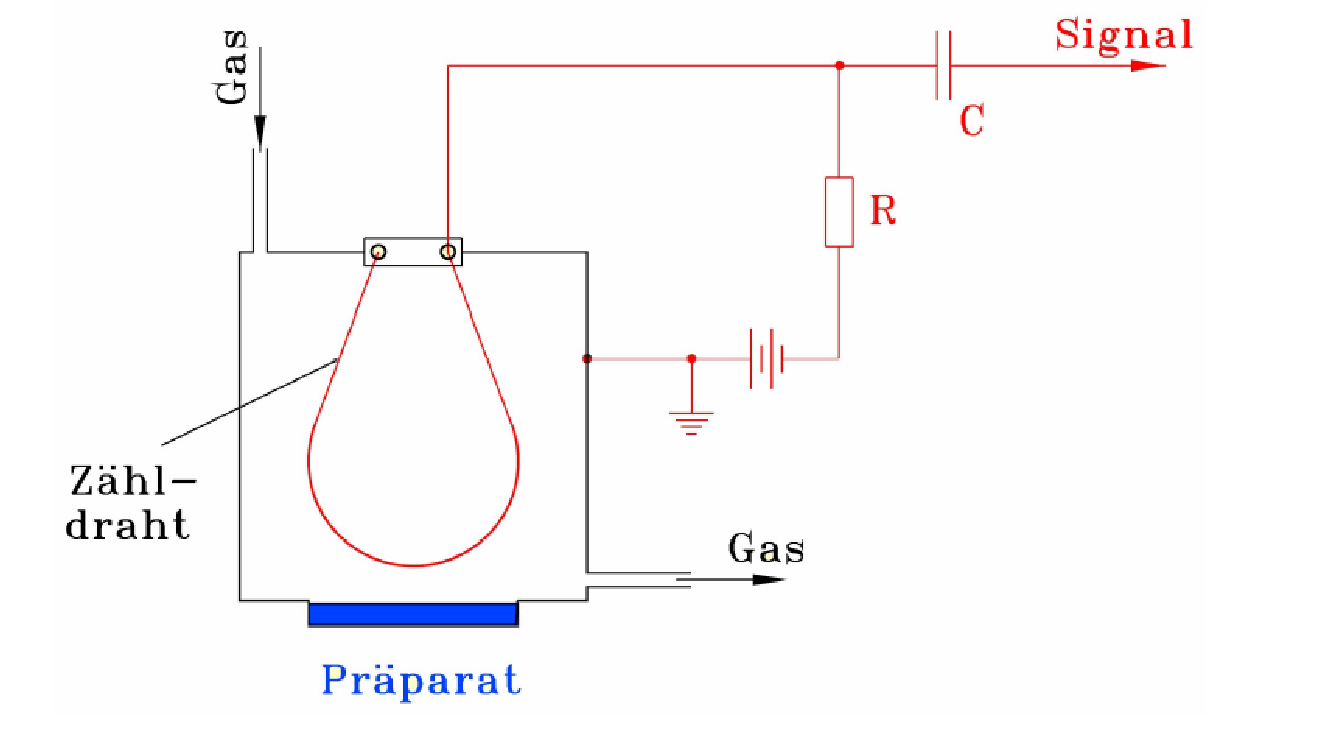
\includegraphics[width=0.9\linewidth]{Bilder/zaehlrohr.png}
 \caption{Aufbau eines Durchflusszählrohrs}
 \label{durchflusszaehlrohr}
\end{figure}
Ein Durchflusszählrohr (siehe Abbildung \ref{durchflusszaehlrohr}) besteht aus einer Zählkammer, die einem normalen Zählrohr ähnelt. Sie besteht also aus einem leitfähigen Kasten und einem Zählring, zwischen denen eine Spannung anliegt. Durch eine Drehvorrichtung kann die Probe direkt in diese Kammer eingebracht werden, wodurch Abschirmungsverluste vermieden werden. Die $\alpha$-Teilchen bzw. Elektronen und Positronen des Zerfalls erzeugen nun einen Strompuls am Ring, der detektiert werden kann. In Abhängigkeit von der Spannung gibt es dabei unterschiedliches Verhalten (vergl. Abb. \ref{theoriezaehlrohrcharakteristik}):
\begin{figure}[h]
 \centering 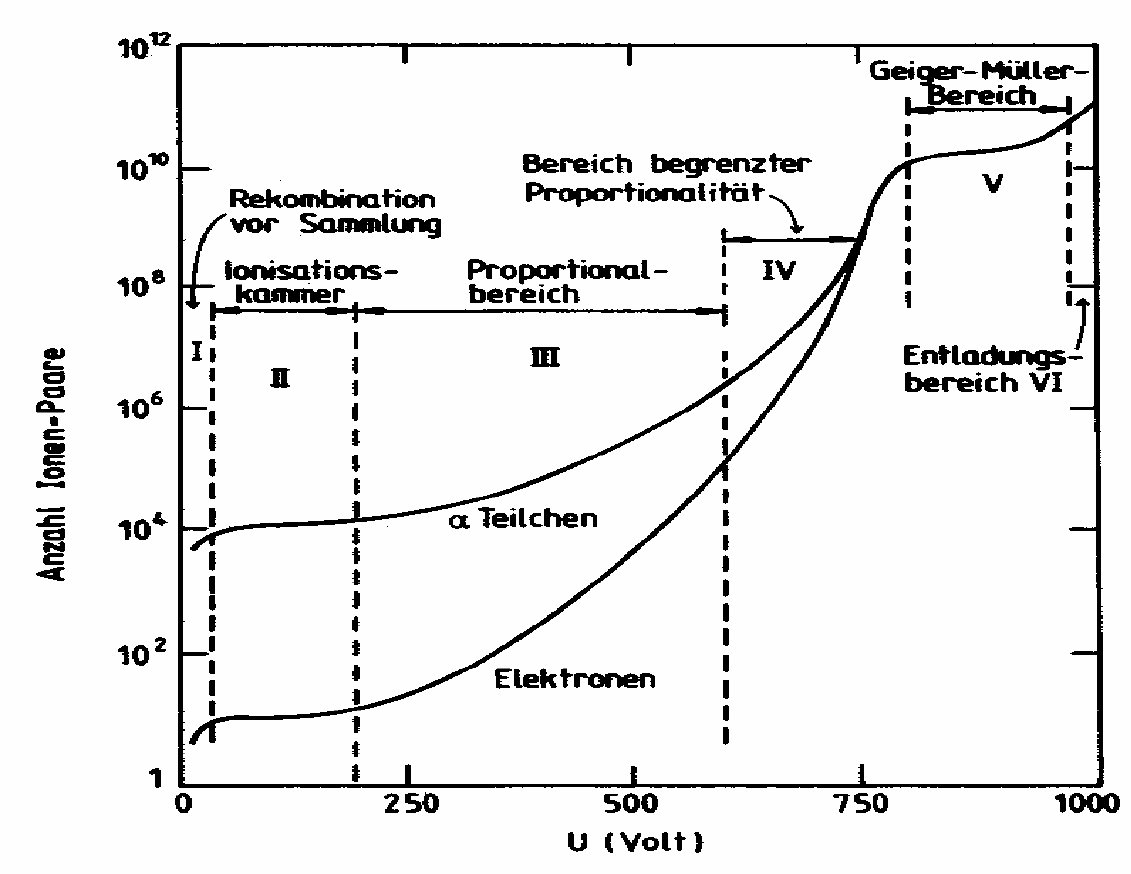
\includegraphics[width=0.9\linewidth]{Bilder/zaehlrohrcharakteristik.png}
 \caption{Typische Zählrohrcharakteristik}
 \label{theoriezaehlrohrcharakteristik}
\end{figure}
\paragraph{Bereich I} Die erzeugten Ionenpaare gelangen nur teilweise bis zum Draht, es kommt meist bereits vorher zur Rekombination. Der gemessene Strom ist hier hauptsächlich von der Spannung abhängig.
\paragraph{Bereich II - Ionisationskammer} Es werden sämtliche Ionenpaare, die durch die Primärionisation entstanden sind, registriert. Man verwendet diesen Spannungsbereich als Ionisationskammer.
\paragraph{Bereich III - Proportionalbereich} Die Ionen aus Primärionisation stoßen mit weiteren Gasmolekülen. Diese werden dadurch ebenfalls ionisiert und es findet eine sogenannte "`Gasverstärkung"' statt. Diese ist proportional zur Energie der Primärteilchen.
\paragraph{Bereich IV} Die Proportionalität zur Primärionisationsenergie wird schwächer.
\paragraph{Bereich V - Geiger-Müller-Bereich} Ein einzelnes Ereigniss löst in diesem Bereich bereits eine Entladungslawine aus und sämtliche Gasatome werden ionisiert. Diese hohe Empfindlichkeit wird im Geiger-Müller-Zählrohr ausgenutzt. 
\paragraph{Bereich VI - Gasentladung} Der Stromfluss bricht in diesem Bereich nicht mehr von selbst ab, ein Zählen der Ereignisse ist somit nichtmehr möglich.

Beim Durchflusszählrohr strömt möglichst konstant ein Gas durch die Kammer, dieses beseitigt verbleibende Ionen vom vorherigen Zählvorgang und verbessert somit die Genauigkeit durch Verringerung der Totzeit und Vermeidung von Fehlzählungen.


